% Copyright 2004 by Till Tantau <tantau@users.sourceforge.net>.
%
% In principle, this file can be redistributed and/or modified under
% the terms of the GNU Public License, version 2.
%
% However, this file is supposed to be a template to be modified
% for your own needs. For this reason, if you use this file as a
% template and not specifically distribute it as part of a another
% package/program, I grant the extra permission to freely copy and
% modify this file as you see fit and even to delete this copyright
% notice. 

\documentclass{beamer}
\usepackage{amsmath,bm}
\usepackage{tikz}
\usetikzlibrary{arrows,automata}
\usepackage{graphicx}

\newcommand{\ssquare}{\text{\scalebox{0.6}{$\square$}}}
\newcommand{\U}{\bm{\mathcal{U}}}


\usepackage{amsmath}
\usepackage{algorithm}
\usepackage[noend]{algpseudocode}

\makeatletter
\def\BState{\State\hskip-\ALG@thistlm}
\makeatother

\floatname{algorithm}{Procedure}
\renewcommand{\algorithmicrequire}{\textbf{Input:}}
\renewcommand{\algorithmicensure}{\textbf{Output:}}


\newcommand{\R}{\mathbb{R}}
\newcommand{\F}{\mathcal{F}}
\newcommand{\Q}{\mathcal{Q}}
\newcommand{\T}{\mathcal{T}}
\newcommand{\A}{\mathcal{A}}
\newcommand{\Inf}{\texttt{Inf}}
\newcommand{\Post}{\texttt{Post}}
\newcommand{\Pre}{\texttt{Pre}}
\newcommand{\Edge}{\texttt{Edge}}
\newcommand{\Cost}{\texttt{Cost}}
\newcommand{\trace}{\texttt{trace}}

% There are many different themes available for Beamer. A comprehensive
% list with examples is given here:
% http://deic.uab.es/~iblanes/beamer_gallery/index_by_theme.html
% You can uncomment the themes below if you would like to use a different
% one:
%\usetheme{AnnArbor}
%\usetheme{Antibes}
%\usetheme{Bergen}
%\usetheme{Berkeley}
%\usetheme{Berlin}
%\usetheme{Boadilla}
%\usetheme{boxes}
%\usetheme{CambridgeUS}
%\usetheme{Copenhagen}
%\usetheme{Darmstadt}
%\usetheme{default}
%\usetheme{Frankfurt}
%\usetheme{Goettingen}
%\usetheme{Hannover}
%\usetheme{Ilmenau}
%\usetheme{JuanLesPins}
%\usetheme{Luebeck}
\usetheme{Madrid}
%\usetheme{Malmoe}
%\usetheme{Marburg}
%\usetheme{Montpellier}
%\usetheme{PaloAlto}
%\usetheme{Pittsburgh}
%\usetheme{Rochester}
%\usetheme{Singapore}
%\usetheme{Szeged}
%\usetheme{Warsaw}

\title{A Discrete B\"uchi Automata Distance for Formal Methods Based Control}

% A subtitle is optional and this may be deleted
%\subtitle{Optional Subtitle}

%\author{F.~Author\inst{1} \and S.~Another\inst{2}}
\author{Garrett Thomas \\
Supervisor: Lars Lindemann \\
Examiner: Professor Dimos V. Dimarogonas}
% - Give the names in the same order as the appear in the paper.
% - Use the \inst{?} command only if the authors have different
%   affiliation.

\institute[Royal Institute of Technology, KTH] % (optional, but mostly needed)
{
  %\inst{1}%
  Automatic Control Department \\
  Royal Institute of Technology, KTH}
  %\and
  %\inst{2}%
  %Department of Theoretical Philosophy\\
  %University of Elsewhere}
% - Use the \inst command only if there are several affiliations.
% - Keep it simple, no one is interested in your street address.

\date{June $28^{\text{th}}$, 2017}
% - Either use conference name or its abbreviation.
% - Not really informative to the audience, more for people (including
%   yourself) who are reading the slides online

\subject{Buchi Distance}
% This is only inserted into the PDF information catalog. Can be left
% out. 

% If you have a file called "university-logo-filename.xxx", where xxx
% is a graphic format that can be processed by latex or pdflatex,
% resp., then you can add a logo as follows:

% \pgfdeclareimage[height=0.5cm]{university-logo}{university-logo-filename}
% \logo{\pgfuseimage{university-logo}}

% Delete this, if you do not want the table of contents to pop up at
% the beginning of each subsection:
\AtBeginSubsection[]
{
  \begin{frame}<beamer>{Outline}
    \tableofcontents[currentsection,currentsubsection]
  \end{frame}
}

% Let's get started
\begin{document}

\begin{frame}
  \titlepage
\end{frame}

\begin{frame}{Outline}
  \tableofcontents
  % You might wish to add the option [pausesections]
\end{frame}

% Section and subsections will appear in the presentation overview
% and table of contents.
\section{Problem and Motivation}

\subsection{Formal Methods Based Control}

\begin{frame}{Linear Temporal Logic}
  \begin{itemize}
  \item {
    We will be using \textbf{Linear Temporal Logic (LTL)}, defined recursively as
    $\varphi ::= \top | \alpha | \neg \varphi_1 | \varphi_1  \lor \varphi_2 | \textbf{X} \varphi_1 | \varphi_1 \bm{\mathcal{U}} \varphi_2$
    \pause
  }
  \item {
    Why?LTL formulas are versatile; LTL allows us to encode statements about the robot and workspace, and also how events relate to each other in the time domain. \\
    Ex. from \cite{guo15} $ \varphi= \diamond(\text{rball} \land \diamond \text{basket}) \land \diamond \ssquare \text{r1}$ \\
    "Eventually pick up the red ball and put it in one of the baskets. Then go home to r1" \\
     \centering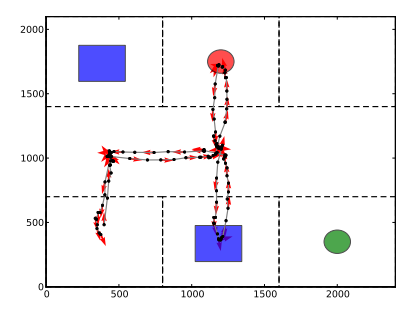
\includegraphics[scale=0.3]{ltlExampleWorkspace}\par
  }
  \end{itemize}
\end{frame}

\begin{frame}{LTL Motion and Task Planning}
	\begin{itemize}	
	\item {
		LTL Motion and task planning is done in three Steps \cite{belta07}
		\pause
	}
	\item<2->{
		Specification: Create a graph (the \textit{product automaton}) based on the workspace, robot motion, and LTL formula such that all paths in this graph satisfy the specification.
	}
	\item<3->{
		Execution: Find a discrete path in this graph using an optimality criterion.*
	}
	\item<4->{
		Implementation: Calculate the continuous controllers such that the continuous path will satisfy the discrete path.
	}
	\end{itemize}	
	
\end{frame}
\subsection{The Product Automaton}

% You can reveal the parts of a slide one at a time
% with the \pause command:
\begin{frame}{Finite-State Transition System}
  \begin{itemize}
  \item<1->{
    The product automaton is the of a \textit{finite-state transition system} and a \textit{B\"uchi automaton}
    \pause % The slide will pause after showing the first item
  }
  \end{itemize}
    \begin{block}{Finite-State Transition System (FTS)}
	\small An FTS is a tuple $\mathcal{T} = (\Pi, \rightarrow, \Pi_0, AP,L_D)$ where $\Pi$ is the set of states, $\rightarrow \subseteq \Pi \times \Pi$ is the transitions, $\Pi_0 \subseteq \Pi$ is the initial state(s), $AP$ is the set of atomic propositions, and $L: \Pi \rightarrow 2^{AP}$ is the labelling function (goes from a state to the set of atomic propositions that are true in that state).
	\end{block}

    
%  \item<5-> {
%    Fifth item. \uncover<6->{Extra text in the fifth item.}
%  }
  \begin{figure}
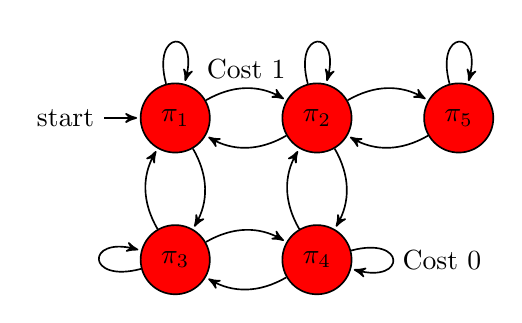
\begin{tikzpicture}[->,>=stealth',shorten >=1pt,auto,node distance=1.8cm,
                    semithick]
  \tikzstyle{every state}=[fill=red,draw=black,text=black]

  \node[initial,state] (A)                    { $\pi_1$};
  \node[state]         (B) [ right of=A] { $\pi_2$};
  \node[state]         (C) [below of=A] { $\pi_3$};
  \node[state]         (D) [right of=C] { $\pi_4$};
  \node[state]         (E) [right of=B] { $\pi_5$};

  \path (A) edge     [bend left]     node {Cost 1}   (B)
  		(B) edge     [bend left]           (A)
		(A) edge     [bend left]         (C)
  		(C) edge     [bend left]           (A)
  		(C) edge     [bend left]         (D)
  		(D) edge     [bend left]           (C)
  		(B) edge     [bend left]           (D)
  		(D) edge     [bend left]           (B)
  		(B) edge     [bend left]           (E)
  		(E) edge     [bend left]           (B)
        (A) edge [loop above]   (A)
        (B) edge [loop above]   (B)
        (C) edge [loop left]   (C)
        (D) edge [loop right]  node {Cost 0} (D)
        (E) edge [loop above]  (E);
\end{tikzpicture}
\end{figure}
\end{frame}

\begin{frame}{B\"uchi Automaton}
\begin{block}{B\"uchi Automaton}
	\small A B\"uchi automaton is a tuple $\mathcal{A}_\varphi = (\mathcal{Q},2^{AP},\delta,\mathcal{Q}_0,\mathcal{F})$ where $\mathcal{Q}$ is a finite set of states, $\mathcal{Q}_0 \subseteq \mathcal{Q}$ is the set of initial states, $2^{AP}$ is the alphabet, $\delta: \mathcal{Q} \times 2^{AP} \rightarrow 2^\mathcal{Q}$ is a transition relation, and $\mathcal{F} \subseteq \mathcal{Q}$ is the set of accepting states.
	\end{block}

	\begin{itemize}
	\item {
	A path on a B\"uchi automaton is accepting if it passes through an accepting state infinitely many times.
	}
	\item {
	For any LTL formula $\varphi$ over $AP$, there exists a B\"uchi automaton over $2^{AP}$ corresponding to $\varphi$ \cite{baier08}
	}
	\end{itemize}
	Reachability while avoiding regions $\varphi = \neg \pi_4 \U \pi_5$
	
	\begin{figure}
\centering
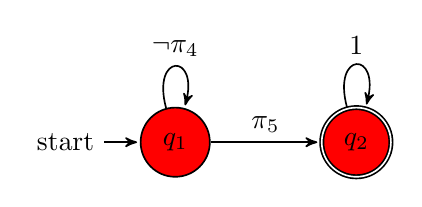
\begin{tikzpicture}[->,>=stealth',shorten >=1pt,auto,node distance=2.3cm,
                    semithick]
  \tikzstyle{every state}=[fill=red,draw=black,text=black]

  \node[initial,state] (A)                    {$q_1$};
  \node[state,accepting]         (B) [right of=A] {$q_2$};

  \path (A) edge              node {$\pi_{5}$} (B)
  		(A) edge [loop above] node {$\neg \pi_4 $} (A)
  		(B) edge [loop above] node {$1$} (B);
\end{tikzpicture}
\end{figure}
\end{frame}

\begin{frame}{Product Automaton}
\begin{block}{Product Automaton}
	\small $\mathcal{A}_p = \mathcal{T}_w \otimes \mathcal{A}_\varphi = (Q', \delta', Q_0', \mathcal{F}', W_p)$, where $Q' = \Pi \times Q = \{ \langle \pi, q \rangle \in Q' | \forall \pi \in \Pi, \hspace{0.2cm} \forall q \in Q \}$; $\delta': Q' \rightarrow 2^{Q'}$. $\langle \pi_j, q_n \rangle \in \delta' (\langle \pi_i, q_m \rangle )$ iff $(\pi_i , \pi_j ) \in \rightarrow_c$ and $q_n \in \delta (q_m, L_d(\pi_j))$; $Q_0' = \{ \langle \pi , q \rangle | \pi \in \Pi_0, \hspace{0.2cm} q_0 \in Q_0\}$, $\mathcal{F}' = \{ \langle \pi, q \rangle | \pi \in \Pi, q \in \mathcal{F}\}$ 
	\end{block}

	\begin{itemize}
	\item {
	Also a B\"uchi automaton
	}
	\end{itemize}
	\begin{figure}
	
\centering
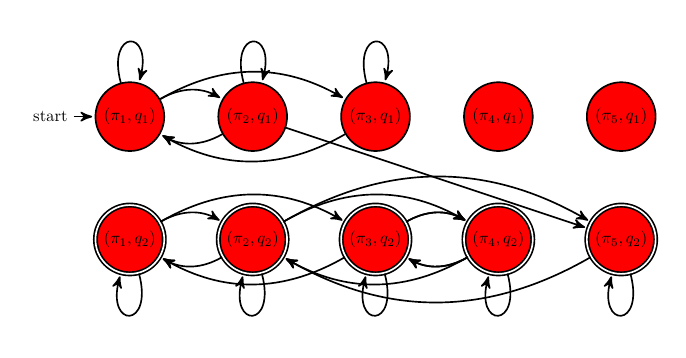
\begin{tikzpicture}[->,>=stealth',shorten >=1pt,auto,node distance=2.6cm,
                    semithick,scale=0.6, every node/.style={transform shape}]
  \tikzstyle{every state}=[fill=red,draw=black,text=black]

  \node[initial,state] (A)                    {$(\pi_1,q_1)$};
  \node[state]         (B) [ right of=A] {$(\pi_2,q_1)$};
  \node[state]         (C) [right of=B] {$(\pi_3,q_1)$};
  \node[state]         (D) [right of=C] {$(\pi_4,q_1)$};
  \node[state]         (E) [right of=D] {$(\pi_5,q_1)$};
  
  \node[state,accepting] 		   (AA)  [below of=A]  {$(\pi_1,q_2)$};
  \node[state,accepting]         (BB) [ right of=AA] {$(\pi_2,q_2)$};
  \node[state,accepting]         (CC) [right of=BB] {$(\pi_3,q_2)$};
  \node[state,accepting]         (DD) [right of=CC] {$(\pi_4,q_2)$};
  \node[state,accepting]         (EE) [right of=DD] {$(\pi_5,q_2)$};  

  \path (A) edge     [bend left]          (B)
        (B) edge     [bend left]          (A)
        (A) edge     [bend left]         (C)
        (C) edge     [bend left]          (A)
        %(C) edge     [bend left]          (D)
        %(D) edge     [bend left]          (C)
		%(B) edge     [bend left]          (D)
        %(D) edge     [bend left]          (B)
        (B) edge               (EE)
        (DD) edge       [bend left]        (BB)
        (BB) edge        [bend left]       (DD)
        (BB) edge        [bend left]       (AA)
        (AA) edge        [bend left]       (BB)
        (BB) edge        [bend left]       (EE)
        (EE) edge        [bend left]       (BB)
        (DD) edge       [bend left]        (CC)
        (CC) edge        [bend left]       (DD)
        (CC) edge        [bend left]       (DD)
        (DD) edge        [bend left]       (CC)
        (CC) edge        [bend left]       (AA)
        (AA) edge        [bend left]       (CC)
        (A) edge [loop above]  (A)
        (B) edge [loop above]  (B)
        (C) edge [loop above]   (C)
        %(D) edge [loop above]   (D)
        (AA) edge [loop below]  (AA)
        (BB) edge [loop below]  (BB)
        (CC) edge [loop below]  (CC)
        (DD) edge [loop below]   (DD)
        (EE) edge [loop below]   (EE);
\end{tikzpicture}

\end{figure}
\end{frame}

\subsection{Execution: Path Finding}
\begin{frame}{Accepted Algorithm}
\begin{itemize}
\item {
	We prefer a prefix, suffix structure $R = \langle R_{pre}, R_{suf} \rangle = q_0' q_1' \dots {\color{red} q_f'} [ {\color{red} q_f'} q_{f+1}' \dots q_n']^\omega$ 
}
\end{itemize}
Here is the algorithm currently used in the literature \cite{guo15},\cite{fainekos09},\cite{kloetzer08},\cite{smith2010}
\begin{algorithm}[H]
\caption{OptRun() \cite{guo15}}
\begin{algorithmic}[1]
\Require Input $\A_p$
\Ensure $R_{opt}$
%\Procedure{MyProcedure}{}
%\State If $Q_0'$ or $\F'$ is empty, construct $Q_0'$ or $\F'$ first.
\State For initial state $q_0' \in \Q_0'$, find the optimal path to each $q_f' \in \F$.
\State For each accepting state $q_f' \in \F'$, calculate the optimal path back to $q_f'$. 
\State Find the pair of $(q_{0,opt}',q_{f,opt}')$ that minimizes the total cost
\State Optimal accepting run $R_{opt}$, prefix: shortest path from $q_{0*}'$ to  $q_{f*}$; suffix: the shortest cycle from $q_{f*}'$ and back to itself.
\end{algorithmic}
\end{algorithm}
\end{frame}

% Placing a * after \section means it will not show in the
% outline or table of contents.
\section{Our Contribution}
\subsection{B\"uchi Distance and Algorithm}
\begin{frame}{B\"uchi Distance Measure}  
  \begin{itemize}
  \item {
    We introduce a discrete B\"uchi distance measure, which is the least number of transitions possible to get to an accepting state 
    \pause
    }
  \end{itemize}
  Ex. Sequencing $  \diamond(\pi_3 \land \diamond \pi_5)$
  \begin{figure}
\centering
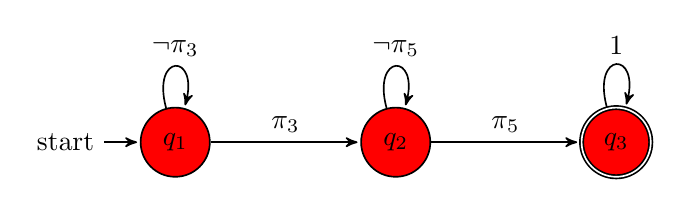
\begin{tikzpicture}[->,>=stealth',shorten >=1pt,auto,node distance=2.8cm,
                    semithick]
  \tikzstyle{every state}=[fill=red,draw=black,text=black]

  \node[initial,state] (A)                    {$q_1$};
  %\node[state] (B)                    [right of=A]{$q_2$};
  \node[state] (B)                    [right of=A]{$q_2$};
  \node[state,accepting]         (C) [right of=B] {$q_3$};

  \path (A) edge              node {$\pi_{3}$} (B)
  		(A) edge [loop above] node {$\neg \pi_3$} (A)
  		(B) edge [loop above] node {$\neg \pi_5$} (B)
  		(B) edge              node {$\pi_{5}$} (C)
  		(C) edge [loop above] node {$1$} (C);
%  		(C) edge              node {$\pi_{3}$} (D)
 % 		(D) edge [loop above] node {$1$} (D);
\end{tikzpicture}
\end{figure}
\pause
\begin{figure}
\centering
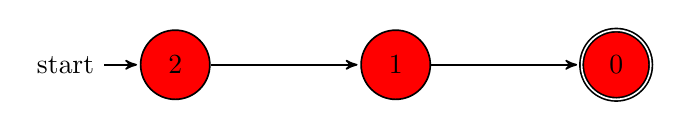
\begin{tikzpicture}[->,>=stealth',shorten >=1pt,auto,node distance=2.8cm,
                    semithick]
  \tikzstyle{every state}=[fill=red,draw=black,text=black]

  \node[initial,state] (A)                    {$2$};
  %\node[state] (B)                    [right of=A]{$q_2$};
  \node[state] (B)                    [right of=A]{$1$};
  \node[state,accepting]         (C) [right of=B] {$0$};

  \path (A) edge               (B)
  		%(A) edge [loop above] node {$\neg \pi_3$} (A)
  		%(B) edge [loop above] node {$\neg \pi_5$} (B)
  		(B) edge              (C);
  		%(C) edge [loop above] node {$1$} (C);
%  		(C) edge              node {$\pi_{3}$} (D)
 % 		(D) edge [loop above] node {$1$} (D);
\end{tikzpicture}
\end{figure}
  \begin{itemize}
  \item {
    Denoted $d_p:\Q \rightarrow \mathbb{Z}$, e.g.\ $d_p(q_2) = 1$ 
    }
  \end{itemize}
\small Note: Transitions with \&\& are removed from LTL2BA because regions do not overlap

\end{frame}




\begin{frame}{Our Algorithm}
\begin{itemize}
\item {
	Motivation for our algorithm: $\mathcal{F}' = \{ \langle \pi, q \rangle | \pi \in \Pi, q \in \mathcal{F}\}$  
}
\item { 
	We greedily find the optimal path which reduces the B\"uchi distance at each step
	}
\end{itemize}
\begin{algorithm}[H]
\caption{GreedyRun()}
\begin{algorithmic}[1]
\Require Input $\A_{p,d}$
\Ensure $R_{g}$
%\Procedure{MyProcedure}{}
\State LEVEL = $d_p(q_0' \in \Q_0')$
\While {LEVEL $> 0$}
\State find optimal path down to $q_n'$ s.t. $d_p(q_n')==LEVEL-1$
\State Level = Level - 1	
\EndWhile
\State Find optimal path from $q_n'$ back to itself
\State Accepting run $R_{g}$, prefix: the optimal paths calculated in the while loop concatenated together; suffix: optimal path from $q_n'$ back to itself.
\end{algorithmic}
\end{algorithm}

\end{frame}

\begin{frame}{Why?}
\begin{itemize}
\item {
	\Large \textbf{We approximate the globally optimal path with a series of locally optimal paths}
}
\item {
	\Large \textbf{We sacrifice a degree of optimality for easier computation!}
}
\end{itemize}
\end{frame}

\section{Performance on Common Formulas}
\subsection{Workspace}
\begin{frame}{Workspace}
\begin{figure}[!htb]
\centering
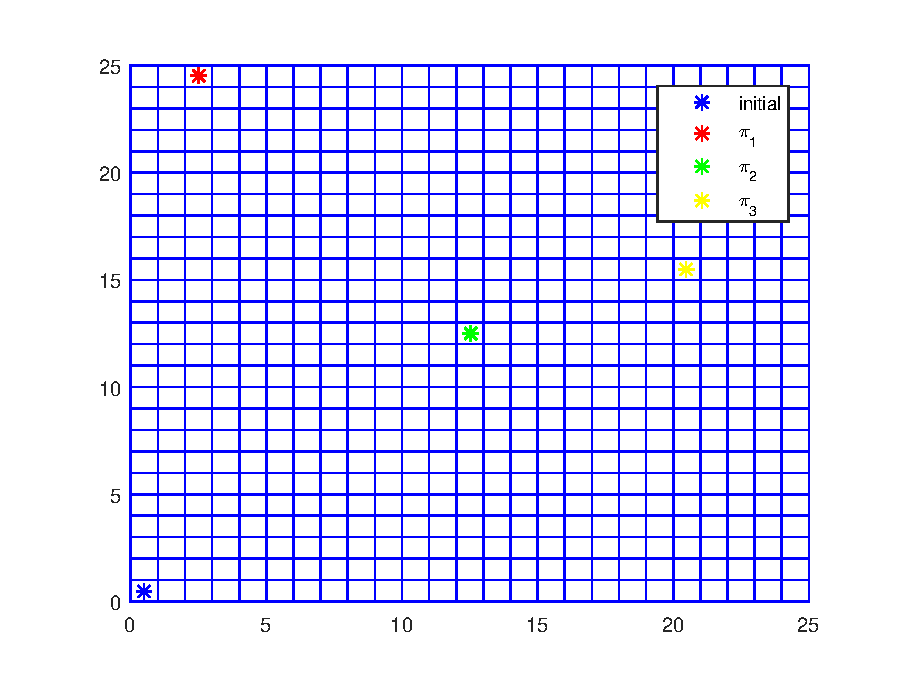
\includegraphics[scale=0.7]{../writing/workspace.eps}
\label{fig:workspace}
\caption{Workspace 1}
\end{figure}
\end{frame}

\subsection{Reachability While Avoiding Regions}
\begin{frame}
\begin{figure}
\centering
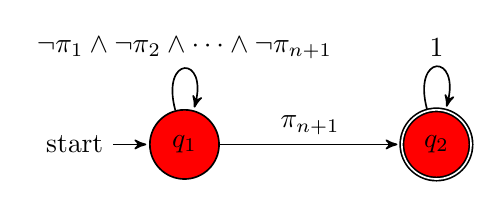
\begin{tikzpicture}[->,>=stealth',shorten >=1pt,auto,node distance=3.2cm,
                    semithick]
  \tikzstyle{every state}=[fill=red,draw=black,text=black]

  \node[initial,state] (A)                    {$q_1$};
  \node[state,accepting]         (B) [right of=A] {$q_2$};

  \path (A) edge              node {$\pi_{n+1}$} (B)
  		(A) edge [loop above] node {$\neg \pi_1 \wedge \neg \pi_2 \wedge \dots \wedge \neg \pi_{n+1}$} (A)
  		(B) edge [loop above] node {$1$} (B);
\end{tikzpicture}
\caption{B\"{u}chi automaton corresponding to $\neg (\pi_1 \lor \pi_2 \lor \dots \pi_n) \U \pi_{n+1}$}
\end{figure}
\centering $d_p(q_1)=1$ and $d_p(q_2)=0$
\end{frame}


\subsection{Sequencing}

\begin{frame}
\begin{itemize}
	\item {
	We look at the sequencing formula $\diamond (\pi_1 \land \diamond(\pi_2 \land \diamond \pi_3))$
	}
\end{itemize}
\begin{figure}
\centering
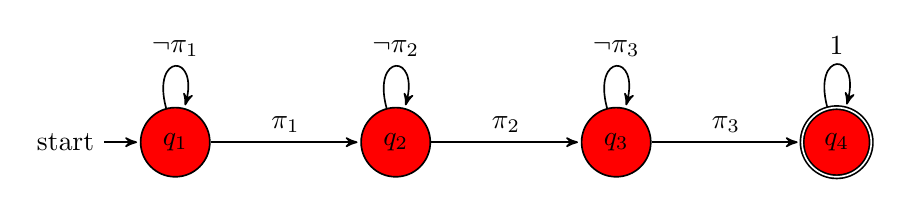
\begin{tikzpicture}[->,>=stealth',shorten >=1pt,auto,node distance=2.8cm,
                    semithick]
  \tikzstyle{every state}=[fill=red,draw=black,text=black]

  \node[initial,state] (A)                    {$q_1$};
  %\node[state] (B)                    [right of=A]{$q_2$};
  \node[state] (B)                    [right of=A]{$q_2$};
  \node[state]         (C) [right of=B] {$q_3$};
  \node[state,accepting]         (D) [right of=C] {$q_4$};

  \path (A) edge              node {$\pi_{1}$} (B)
  		(A) edge [loop above] node {$\neg \pi_1$} (A)
  		(B) edge [loop above] node {$\neg \pi_2$} (B)
  		(B) edge              node {$\pi_{2}$} (C)
  		(C) edge [loop above] node {$\neg \pi_3$} (C)
  		(C) edge              node {$\pi_{3}$} (D)
  		(D) edge [loop above] node {$1$} (D);
\end{tikzpicture}
\caption{B\"uchi Automaton Corresponding to $  \diamond(\pi_3 \land \diamond \pi_5)$}
\end{figure}
\end{frame}


\begin{frame}[allowframebreaks]
	%\begin{thebibliography}{10}
        \frametitle{References}
        \bibliographystyle{amsalpha}
        \bibliography{../writing/bibliography}
     %\end{thebibliography}
\end{frame}

\end{document}